\chapter{GEMINI overzicht}
\label{gemini_beschrijving}

GEMINI is een applicatie voor de flexibele analyse van genoomdata van populaties van menselijke individu\"en. Deze sectie gaat dieper in op de belangrijkste features en het onderliggende datamodel van GEMINI in zijn oorspronkelijke vorm \cite{10.1371/journal.pcbi.1003153}\cite{gemini_docs}.

\section{Database schema}

GEMINI importeert genetische variants en genotypes van alle gesampelde individu\"en (ook 'samples') vanuit een VCF file in een relationele database.
Daarnaast kan extra informatie over de samples, zoals geslacht, phenotype en onderlinge verwantschappen, meegegeven worden in een PED-file (van pedigree) om latere analyse te vergemakkelijken.\\

Elke variant in een input VCF file wordt uitvoerig geannoteerd na automatische vergelijking met bestaande of door de gebruiker gedefinieerde genoom-annotatiebestanden. De geannoteerde variants vormen de rijen van de hoofdtabel van de database, de \texttt{variants}-tabel. Deze tabel bevat ook voor elke variant informatie over elke sample, zoals diens genotype, de kwaliteit en diepte van de meting voor de variant in kwestie. In de SQLite-versie van GEMINI wordt dit opgeslagen als een gecomprimeerde array per variant, 1 voor elke sample-eigenschap: zo is er een \texttt{gt\_type}-kolom met arrays met de genotypes, en een \texttt{gt\_depth}-kolom met arrays met de diepte van de meting van elke sample voor elke variant. Samen met de \texttt{samples}-tabel, die voor elke sample zaken als het geslacht, phenotype en familierelaties bijhoudt, ligt de \texttt{variants}-tabel aan de basis van de uitgebreide query-mogelijkheden die GEMINI biedt.\\

Daarnaast zijn er nog tabellen zoals de \texttt{variant\_impacts}- en \texttt{gene\_detailed}-tabellen die respectievelijk extra informatie over de variants en het menselijk genoom bevatten. Deze informatie komt in het eerste geval eveneens uit de annotatiebestanden, en in het tweede uit tekstbestanden met referentie-informatie over het menselijk genoom die GEMINI, indien gewenst mee inlaadt.\\
Ten laatste zijn er nog enkele kleine tabellen met meta-informatie, zoals de \texttt{resources}-tabel die de gebruikte annotatie-files bevat, en de \texttt{version}-tabel die bevat door welke versie van GEMINI de data ingeladen is.\\

\begin{figure}[!h]
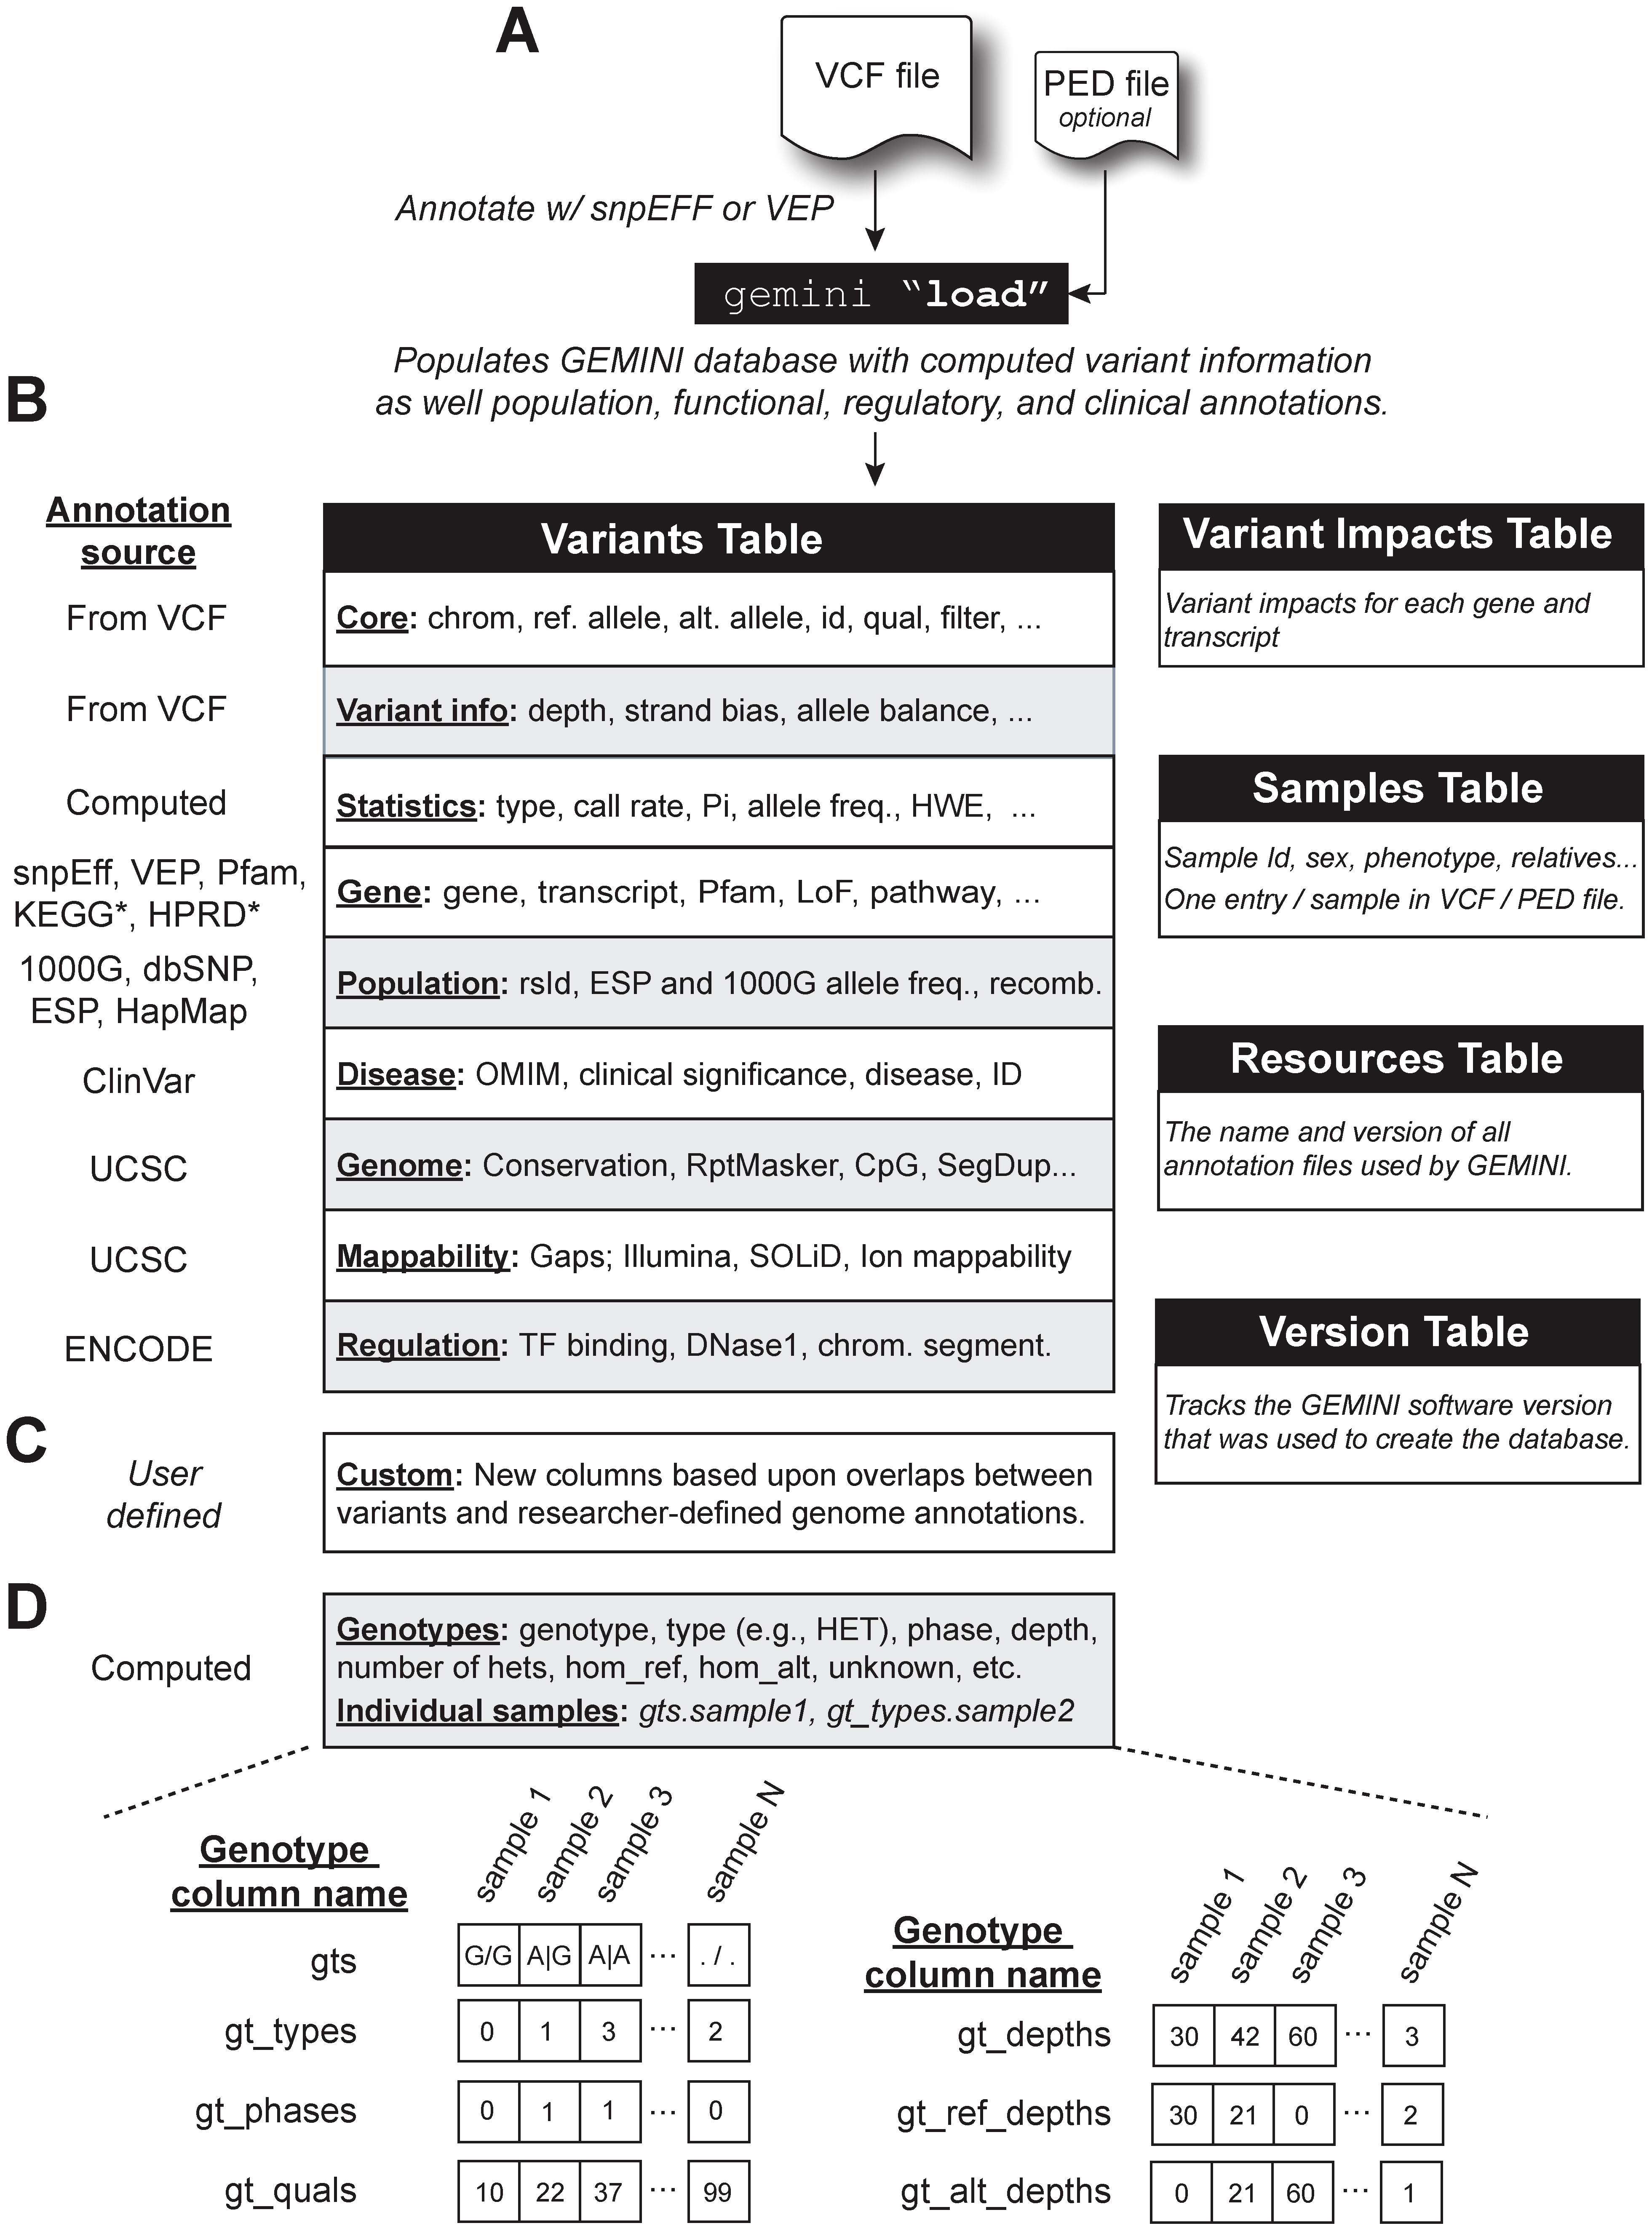
\includegraphics[width=\textwidth,height=\textheight,keepaspectratio]{gemini_schema}
\caption{Een overzicht van GEMINI's schema}
\label{gemini_schema_pic}
\end{figure}

Een belangrijke troef van GEMINI en z'n datamodel is de flexibiliteit die het laat naar de gebruiker. Zo kan de gebruiker zelfgedefinieerde annotatie-files gebruiken, en zelf kolommen toevoegen aan de PED-files met informatie over de samples. Deze extra informatie zal GEMINI automatisch in de resp. \texttt{variants}- en \texttt{samples}-tabel opnemen en kan de gebruiker later ook doorzoeken.\\

Figuur \ref{gemini_schema_pic} schetst een overzicht van de structuur van GEMINI.


\section{Inladen}
Het inladen van de data uit VCF-bestanden is een computationeel intensieve operatie, enerzijds omwille van de enorme grootte van deze bestanden, en anderzijds omdat in deze fase ook alle variants geannoteerd moeten worden. Om het proces te versnellen, biedt GEMINI de mogelijkheid het werk te paralleliseren door het VCF-bestand de comprimeren, op het bestaande bestand een index te defini\"eren en zo het werk te verdelen. Dit kan over meerdere processoren binnen 1 computer zijn, maar via de IPython-interface ook over volledige clusters van computers \cite{PER-GRA:2007}.\\

\section{Querying}

GEMINI laat de gebruiker toe de opgeslagen genoomdata te doorzoeken. Enerzijds via gewone SQL-queries, maar omdat het onderzoeken van individuele genotypes van cruciaal belang is in het onderzoek naar ziektes en SQL standaard niet de individuele genotypes in array-kolommen kan opvragen, biedt GEMINI bovendien een verrijkte SQL-syntax.\\
Zo laat het de gebruiker toe via filters en wildcards de gewenste genotype-eigenschappen en samples te specifi\"eren.

\subsection{Sample filters/wildcards} 
In SQL \texttt{SELECT}-statements kan de gebruiker met een filter van de vorm column.sample of een wilcard van de vorm (column).(wildcard) uitdrukken welke genotype-kolommen van welke samples hij/zij wilt zien. Wanneer de gebruiker ge\"interesseerd is in bijvoorbeeld het genotype van Jan, wordt dit:\\
\texttt{SELECT gt\_types.Jan FROM variants}\\\\
Als de gebruiker de diepte van de genotypes alle samples van vrouwelijke proefpersonen wil zien, wordt dit:\\\\
\texttt{SELECT (gt\_depths).(sex = 'female')}.\\
GEMINI vertaalt de wildcard automatisch naar een query op de \texttt{samples}-tabel, en kan vervolgens voor alle samples die aan de voorwaarden voldoen, de waarde uit de gevraagde kolom tonen.

\subsection{Genotype filters/wildcards}
Om beperkingen op te leggen aan de variants waarin hij ge\"interesseerd is, kan de gebruiker SQL \texttt{WHERE}-clausules uitbreiden met zogenaamde genotype filters. Is de gebruiker bij voorbeeld enkel ge\"interesseerd in variants waarvoor John heterozygoot is en Alex alles behalve heterozygoot is, kan dit met:\\

\noindent\texttt{\$ gemini query -q} "\texttt{SELECT * FROM variants}"\textbackslash \\\texttt{--gt-filter }"\texttt{gt\_types.John == HET and gt\_types.Alex != HET}"\\

\noindent Vaak is het de bedoeling om eenzelfde beperking op te leggen aan meerdere samples. Op bovenstaande manier wordt dit voor een toenemend aantal samples al snel pijnlijk veel en foutgevoelig werk. Om dit te verhinderen, zijn er genotype wildcards van volgend formaat:\\ 
\texttt{(column).(sample\_wildcard).(gt\_wildcard\_rule).(rule\_enforcement)}.
\begin{description}
\item[column] Staat voor de genotype kolom waarop de beperking slaat.
\item[sample\_wildcard] Een wildcard om aan te duiden voor welke samples de beperking moet gelden. Analoog met de eerder vermelde sample wildcards.
\item[gt\_wildcard\_rule] De beperking op de genotype kolom.
\item[rule\_enforcement] Duidt aan hoeveel van de geselecteerde samples aan de opgelegde gt\_wildcard\_rule moeten voldoen. Dit kan \texttt{all, any, none, of count <comparison>} zijn.
\end{description}

\noindent Alle variants opvragen waarvoor alle mannelijke proefpersonen heterozygoot zijn, gaat bijvoorbeeld met:

\noindent\texttt{\$ gemini query -q "}\texttt{SELECT * FROM variants"}\textbackslash \\
\texttt{--gt-filter" }\texttt{(gt\_types).(sex = 'male').(=HET).(all)"}\\

\noindent Alle variants opvragen waarvoor minstens 1 bruinharig individu een genotype van diepte minstens 100 heeft, met:

\noindent\texttt{\$ gemini query -q "}\texttt{SELECT * FROM variants"}\textbackslash \\
\texttt{--gt-filter" }\texttt{(gt\_depths).(hair\_colour = 'brown').(>=100).(any)"}\\

\noindent Alle variants opvragen waarvoor minder dan 10 individu\"en een genotype met diepte minder dan 50 hebben, met:

\noindent\texttt{\$ gemini query -q "}\texttt{SELECT * FROM variants"}\textbackslash \\
\texttt{--gt-filter" }\texttt{(gt\_depths).(*).(=HET).(count < 10)"}\\

\noindent Al de bovenstaande filters kunnen met elkaar gecombineerd worden, evenals met gewone WHERE-clausules op de andere kolommen van de variants-tabel.

\subsection{\texttt{--show-samples}}

GEMINI biedt ook de mogelijkheid, bij een query op de \texttt{variants}-tabel, voor elke variant die aan de gestelde eisen voldoet, de namen van alle samples weer te geven die voor gegeven variant homozygoot of heterozygoot zijn. Dit gebeurt door de \texttt{--show-samples} flag mee te geven aan het \texttt{query} commando.



